\documentclass[ecp,tc,english]{iiufrgs}
% 
% Outras Opções:
% * english    -- para textos em inglês
% * openright  -- Força início de capítulos em páginas ímpares (padrão da
% biblioteca)
% * oneside    -- Desliga frente-e-verso
% * nominatalocal -- Lê os dados da nominata do arquivo nominatalocal.def


\usepackage[utf8]{inputenc}   % pacote de acentuação unicode
\usepackage{graphicx}         % pacote de importar figuras
\usepackage{times}            % pacote de fonte Adobe Times
\usepackage{fixmath}          % pacote de math international standardization
\usepackage[alf,abnt-emphasize=bf]{abntex2cite}	% pacote de citações abnt
\usepackage{subcaption}

\newtheorem{definition}{Definition}

\title{From Timeout-based to Item-by-Item Analysis: Investigating Methodologies for Splitting User Sessions Originated from Shared Accounts in Online Platforms}

\author{Tura}{Matheus Toazza}
\advisor[Prof.~Dr.]{Cordeiro}{Weverton Luis da Costa}
\coadvisor[Prof.~Dr.]{Galante}{Renata de Matos}
\location{Porto Alegre}{RS}
\date{May}{2021}

\keyword{Dimensionality reduction}
\keyword{clustering}
\keyword{user profiling}
\keyword{session identification}
\keyword{recommendation systems}

\begin{document}

\maketitle

\begin{acknowledgements}
First and foremost, I would like to dedicate this work to my parents Genir and Lurdes that supported me during my development as graduate student, and to my friend Dennis Balreira that helped me on the most difficult storms from hard and demanding disciplines and also to my homeless friend Paulo, that used to encourage me to finish my degree every time I used to see him on streets.

I am deeply grateful to my advisor, Weverton Cordeiro for his profissionalism and clarity on the way he guided me trough and also to my co-advisor Renata Galante that faded any misdirection with wisdom.

Special thanks to Carolina Nery that helped me with discussions and insights during the construction of this work.
\end{acknowledgements}

% dedicatoria
\clearpage
\begin{flushright}
    \mbox{}
    \vfill
    {\sffamily\itshape
      ``Nothing in life is to be feared, it is only to be understood.\\
      Now is the time to understand more, so that we may fear less.''\\}
    --- \textsc{Marie Curie}
\end{flushright}

% TODO ponctuate the difference that you are using a content-only timeless technique
\begin{abstract}
  Although some content providers register stream data from its users and can track their profile style for content recommendation, when two or more users share a same account, their true profile activity is obfuscated and fuzzed, this user behavior hinders the recommendation systems from providers, moreover, the growing concerns on user privacy poses a risk to current models that rely on unconcealed user identity. This work proposes a way of classifying users' stream data trough sessions, based only on its media content, opening the possibility for breaking a same account profile within multiple user profiles and consequently identifying this activity. In this work dimensionality reduction and clustering methods are used to classify user stream data into sessions that correspond to each respective user profile.
\end{abstract}

% resumo em português
\begin{englishabstract}{}{Redução de dimensionalidade, Clusterização, Perfis de usuários, Identificação de sessões, Sistemas de recomendações}

  Embora as provedoras de conteúdos registram dados de acessos de seus usuários e consigam analisar seus perfis para recomendações de conteúdo, quando duas ou mais pessoas compartilham da mesma conta a atividade e perfil original e individual de cada usuário é obfuscada e difusa por essas contas compartilhadas, este comportamento confunde os sistemas de recomendação existentes, além disso, o aumento da preocupação com a privacidade dos usuários coloca em risco os modelos atuais que são dependentes de reconhecimento explícito dos usuários.
  Este trabalho propõe uma maneira de classificar o fluxo de dados dos usuários em sessões baseando-se apenas em seu conteúdo, abrindo portas para quebrar a mesma conta em múltiplos perfis de usuários e consequentemente identificando esta atividade. Neste trabalho Redução de dimensionalidade e métodos de clusterização são utilizados para classificar o fluxo de dados em sessões que correspondem respectivamente a cada perfil de usuário.
\end{englishabstract}

\listoffigures 
\listoftables 

\begin{listofabbrv}{SPMD}
    \item[PCA] Principal Component Analysis
    \item[SNE] Stochastic Neighbor Embedding
    \item[SVD] Singular Value Decomposition
    \item[tSNE] t-Distributed Stochastic Neighbor Embedding
    \item[EM] Expectation-Maximization Clustering
    \item[RNN] Recurrent Neural Networks
    \item[ALS] Alternating Least Squares    
    \item[CF] Colaborative Filtering
    \item[CB] Content-based Filtering
\end{listofabbrv}

\tableofcontents % sumario

% =======================================================================

%TODO No final da introdução atualizar o paragrafo que explica brevemente cada capítulo.  
\chapter{Introduction}
Most platforms nowadays rely on recommendation systems to create plug and play interactions between users and offered items, avoiding search time and making platform navigation minimal and crisp, however, some user behaviours or even the emerging privacy laws and growing concerns on data privacy, recommendation systems precision can get affected by profiling contamination on the user-item relations  and its interpretation by the system.

One commonly known example responsible for grinding the recommendation systems performance is the practice of account sharing that mixes and masks its account profiles against its real users. Account sharing behaviour is non-intentional in most cases, since device sharing is common, there could be a situation where some individual into his computer is searching videos in a logged-in streaming platform for specific subjects like for example C++ usage, but at some point, it leaves the computer empty without performing account logout, another individual then starts using the same device and platform but for a completely different subject, like children's cartoon.

This problem is evident on commonly used time-based session identification techniques such as \cite{halfaker2015}, the presented scenario would fail in identifying sessions, if chosen period threshold for breaking sessions is long enough, the elapsed time from user permutation usage on platform could be insignificant on the total session time, thus preserving the unity of the session, but in reality two completely sessions have happened during this period.

On \cite{jiang2018} its main goal is identifying shared accounts in multimedia streaming and it addresses a clearly domain separation between \textit{account-level recommendation} and \textit{user-level recommendation}, but even so, they use a timeout along with their other techniques to break the session.

The proposed work consists in two global objectives: (i) Verifying the possibility of an algorithm for session identification based on item category instead of timeout, 
(ii) Create an evaluation method for reliably testing its accuracy and precision.

\textit{globo.com} dataset offered a good amount of data, it was preferred instead of others due to it's availability and data abundance, however, since they do not allow the use of news content, \cite{moreira2018chameleon} made available its embeddings that carries 250 dimensions of features for each of more than 300,000 articles, also \textit{globo.com} dataset aggregates streams of user clicks with more than 2.8 millions of clicks with labeled information such as user\_id and timestamp; the attribute of stream click is addressed at section \ref{globo_dot_com_dataset}.
Dimensionality reduction technique was needed in order to reduce complexity of data and apply the \(Affinity Propagation\) clustering algorithm. 

Two main methods of evaluation are addressed, the first is an \textit{euclidean distance} based method were the distance between each article content is considered; the second evaluation method relies on \textit{matrix factorization} such as ALS technique \cite{takane1977} where read frequency from labeled news topics acts as an implicit correlation from users to items.

The image below describes in general terms the pipeline of both proposals

\begin{figure}[H]
    \centering
    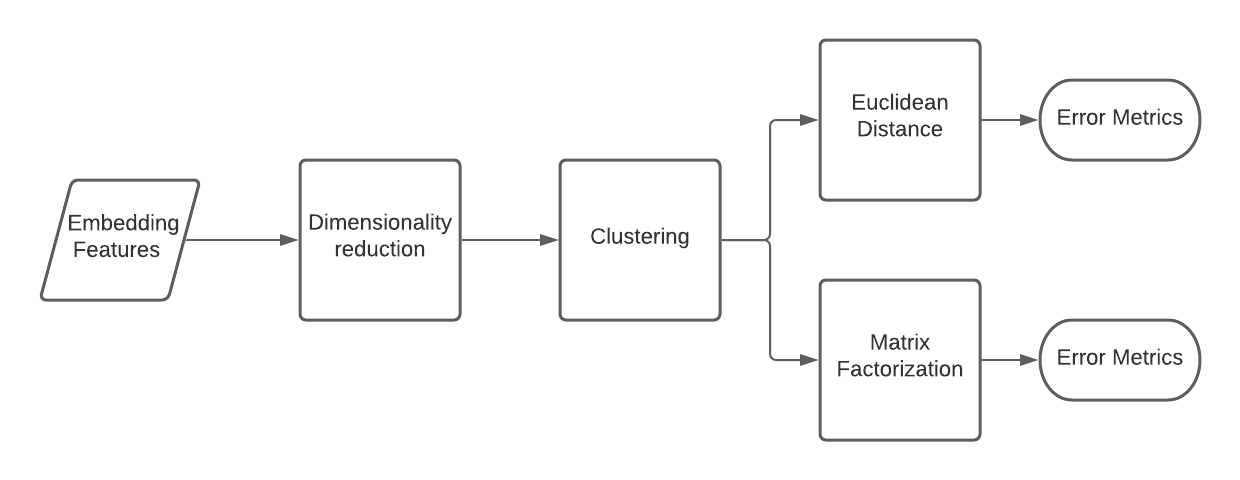
\includegraphics[width=0.9\textwidth]{images/experiment.png}
    \caption{Proposed validation method}
    \label{fig:method_architecture}
\end{figure}

%TODO Está um pouco genérico, especificar alguns pontos.
This work is organized as follow: Initially on chapter \ref{theoretical_background_and_related_work} basic concepts and methods needed to fulfil the following reasoning are introduced, later related works on chapter \ref{related_works} that backed the choices made on this project. On the chapter \ref{methodology} the session problem modelling is introduced and described as well as known problems for multidimensional data and its manipulation. The section \ref{algorithms} that follows introduce solutions for the defined problems.
Finally, on chapter \ref{results} error measurement modeling is addressed along with it metrics results.

% =======================================================================

\chapter{Theoretical Background} \label{theoretical_background_and_related_work}
Here you will find the foundations for this work, they will be introduced as well as related works, those are crucial to assemble the complete picture.

At subsection \ref{basic_concepts}, basic concepts and attributes are introduced and on subsection \ref{dimensionality_reduction} and \ref{cluster_analysis} methods and algorithms are introduced with its applicability and past usage. Related works are presented on subsection \ref{related_works}

    \section{Basic concepts} \label{basic_concepts}
        \begin{itemize}
            \item \(User\) is the person itself that is using the platform trough an account, most of times each user has its own account, but at sometimes, one account can have multiple users.        
            \item \(Account\) is a platform gateway and record that contains user detailed information and is used to register user history associating each requested item with its requester account id.
            \item \(Item\) represents the consumed media, can be music, image, video or text in case of a news article.
            \item \(Clickstream\) is a group of requested items ordered by request timestamp.    
            \item \(Session\) is a subset of a \(clickstream\), the beginning and end of a session are commonly tagged considering user idleness, where the time difference between one requested item and the next one is higher than a certain period threshold, however, the proposed method is timeless and take in account only content categories as a session split threshold.
        \end{itemize}

        % User and Account
        An account is the common gateway for an user to access the platform content, most of past works consider that each account is in fact one user which may happen on most scenarios because normally each user has its own account, but sometimes and even more on paid platforms, an account is shared between more users.
    
        % Item and Session        
        An item is a pair with a click timestamp and a media id identification. 
        At Globo dataset, each item is a  set \((timestamp, click\_id)\) but 
        in any other dataset, the click id is a reference to news, music, 
        image, video or any metadata associated. A session is a well defined 
        segment from a stream of items from one account. There are many ways 
        of defining session boundaries, on \cite{arlitt2000} the session 
        is defined by using time threshold, same as \cite{halfaker2015}. 
        For example when a user stays inactive for an amount of time, that can be 
        considered an end of a session and start of another. In this proposal the 
        sessions will be split considering the content type in order to identify 
        account sharing or even user profiling for different user tastes.


        \section{Recommendation system}
        The role of a \textit{recommendation system} is to make inferences of new \(items\) that the \(user\) would like and suggest them. It is a set of algorithms that together they can return for example an ordered list of probability/similarity from items that were previously compared against other items. These other items must be similar from the ones that the \(account\) have interacted or similar accounts have interacted with.
        Variables such as click-rate, visit frequency, time spent on page can be considered to calculate an affinity between interacted \(items\) and \(account\).

        A recommendation system can have four main classifications:
        \begin{itemize} 
            \item Implicit vs Explicit
            \item Content-based vs Collaborative
        \end{itemize}

        \textit{Implicit vs Explicit} definitions correspond to the way data is semantically related between the pair \(account\)-\(item\). On \(Implicit\) recommendation systems there is an implicit relationship between the used item and the expectation that the majority of those items are desirable by its user, on the other side of the spectrum, there are the \(Explicit\) recommendation systems that usually uses a rate system given by the \(user\), so there is not just a simple link between both entities, but also a subjective magnitude that could be either positive or negative, qualitatively speaking.

        \textit{Content-based vs Collaborative} classifies on an \(account\)-\(account\) relationship. On the first one the similarity between interacted items on a same account is used to retrieve similar new items that the user didn't yet explored, on the second one, the comparison is based upon other accounts that share similarity, so items from these accounts that are missing on the interaction history can be recommended. On state of art systems, both methods are combined in order to get the best results.    
        
        % TODO subseção com apenas 2 parágrafos
        \section{Dimensionality reduction} \label{dimensionality_reduction}
        The more dimensions a data has the more diluted the statistical significance becomes, 
        because data sparsity grows exponentially as the dimensions grow linearly,  
        this phenomena is called \textit{the curse of dimensionality} and is described on \cite{marimont1979} and one on way to finding statistical significance are techniques of \textit{dimensionality reduction}, further discussions and solutions are discussed on \ref{data_scarcity_and_sparcity}.
        
        One of firsts successful algorithms for this purpose is called \textit{Principal Component Analysis} 
        by \cite{hotelling1933} and it consists in finding linear combinations between pair of dimensions that corresponds to most statistical significance trough variance, where the two most significant linear combinations becomes the main dimensions and its points are plotted in a two dimensional Cartesian plane.
        Dimensionality reduction techniques are used before applying Clustering algorithms, because normally media contents are described as an array of multidimensional features.
        
        Since media content normally arrives in image, sound or text, content classification is a multidimensional case, those types of data are rich in both syntactic and semantic information, the common pipeline of classification rely on techniques of feature extraction following dimensionality reduction, however, this type of content are not made of linear combinations problems, but non-linear relationships between dimensions, for this purpose several techniques rather than PCA (that is linear by its nature) were developed on the past. For the purpose of this work, given the non linearity of news embeddings and as mentioned on \cite{moreira2018chameleon}, provider of the dataset embeddings used on this work, tSNE method from \cite{maaten2008} was considered as the best approach; this technique uses \textit{gradient descent} \cite{bryson1962} to minimize \textit{relative entropy} \cite{kullback1951} from distance distributions between all combinations of pairs from the data points; in fact, those distributions are the euclidean distance from each point against others and each distance projected into a distribution function, the innovative difference between tSNE and its predecessor SNE \cite{hinton2002} is that it uses t-student distribution instead of gaussian, that is far more cheaper computationally and generates similar but denser results.
        
        % TODO subseção com apenas 1 parágrafo
        % TODO why affinity propagation? what about other methods?
        \section{Cluster analysis} \label{cluster_analysis}
        It is the method for grouping items that share a vicinity/similarity and then labelling each one of the groups, normally, clustering algorithms are applied on points plotted on two or three dimensional planes. There are many types of clustering algorithms but for the construction of four main used types of algorithms were taken into account describe below:
        
        \begin{itemize} 
            \item \textbf{Centroid-based}
            
            One of the oldest clustering algorithms is k-means \cite{steinhaus1956, macqueen1967}, \(k\) is the number of clusters pick at the beginning of the algorithm, than \(k\) randomly cluster centers are introduced into the set of points, it is attributed each point to the closest cluster center in respect to it's euclidean distance, this process is repeated many times as necessary to reduce the variance between each cluster points, however, the problem of this kind of algorithm is that the user must test the \(k\) parameter multiple times till it find the best fit, \textit{Affinity-propagation} algorithm  \cite{frey2007} on the other hand, it doesn't know previously the quantity of cluster centers, it is discovered during the calculation, for that reason \textit{affinity propagation} was chosen for the proposed method. 
            
            \item \textbf{Distribution-based} 
            
            This clustering category works as a soft clustering, since during calculation it attributes for every point it is assigned a probability of ownership from each individual cluster, in every step of calculation, those probabilities are update and in the end, the point is claimed by the cluster which it has the biggest probability of ownership.
            
            The most used distribution-based algorithm is \textit{EM clustering} from \cite{dempster1977} where the mentioned steps are split into \textit{Expectation (E)} steps followed by \textit{Maximization (M)} steps in alternation between each other, it can be viewed also as an \textit{relative entropy} reduction problem \cite{kullback1951} between the expected distribution and the resulting distribution.
            
            \item \textbf{Density-based}
            
            It is based on the concept of "density-reachability"; the most used density-based method is DBSCAN \cite{ester1996}, where euclidean distance is used as a radius from the observed point, where every neighbor point inside its radius is "contaminated" by its cluster label, the problem of this kind of method is when you have homogeneous density of points or a smooth transition of density from on cluster to another, this can mislead the algorithm. DBSCAN complexity has a \(O(n\ log\ n)\) average complexity. It is commonly used for unsupervised learning and anomally detection.
            
            \item \textbf{Hierarchical-based}
            
            They are divided into \textit{agglomerative} and \textit{divisive} categories, on the first, it merges small clusters into big clusters, on the second one, it keep subdividing from one big starting cluster to more small clusters, they are mainly used for genetics and species classification and two famous methods are \textit{single-linkage} and \textit{complete-linkage} \cite{johnson1967, sibson1973} clustering. Hierarchical clustering algorithms are considered very slow since they have quadratic or cubic complexity, for that reason this type of clustering method was not chosen for the proposed work.
        \end{itemize}

% =======================================================================

\chapter{Related works} \label{related_works}
There were a clear distinction between timeout, time-decay and profile-based models on account sharing and user identification related works, for that reason, they are presented as follow divided by three addressed categories as timeout, time-decay and profile-based methods.

\section{Timeout models}

An attempt to categorize user sessions at Youtube platforms, \cite{gill2008} made a distinction between user level and session level characterization, its definition of session beginning and end is a timeout fashion and the explanation for this is that analyzing traffic network is challenging because most of times there is no clear registry of login and logout. They used a benchmark technique to define what is the best time threshold that would really define a session; they found out that 40 minutes of inactivity as threshold is the spot because from this point on, the number of sessions starts to level-off considerably.
Nonetheless, they do not take into account multiple users swapping use like scenarios were a computer can have a very fast turn over, like lan-houses or public spaces with computers or even paid multi-platform account sharing such as \url{togetherprice.com} and \url{kotas.com.br}.

% 1 Hora
One example of account decomposition is \cite{bajaj2016} that individualize each user as a  persona from online TV platforms accounts. Account sharing is very common between families  in front of a TV. This persona-based individualization uses TV logs to generate user profiles; cosine similarity is applied on item frequency matrices that later are clustered using hierarchical clustering where each cluster is an account, lastly, they use their \(Apriori\) algorithm to categorize each persona, however, their session categorization is based on hourly inactivity timeout and their technique is restricted to TV platforms.

% 30 minutes
The work \cite{halfaker2015} consists in clickstream monitoring of different domains on online activity browsing (games, search engines, page views), thus achieving session identification using a fixed 30 minutes inactivity threshold as session identification, authors demonstrates high regularity between different sessions from a same user. 
Since they do not address account sharing, there is a chance that threshold based on item usage or user behaviour instead of time usage, would have more impact on identifying sessions related to different users.

% 30 minutes
A state of art contribution is described on \cite{jiang2018} that using the \textit{LastFM} and \textit{KKBOX} datasets, they address a solution on user identification on shared accounts at streaming platforms given its history logs, proposing the novel unsupervised learning SHE-UI, they could be able to identify groups of users sharing a same account, bringing their solution to an user-level recommendation domain instead of account-level, however, there is a pre-processing step on the stream of items that split sessions based on 30 minutes user inactivity and not based on its content, so people using the same account on different computers with IP obfuscation techniques wouldn't be taken into account for example.


\section{Time-decay models}

% time-decay, time window de 30 minutos
A common method on recommender systems for defining subsets from stream data is introducing decaying weights on items in respect to time, \cite{sottocornola2018} addresses the absence of session delimitation, their technique introduce a time sliding window, they deal with data sparsity using the hibrid approach, combining both CF and CB; they delimit each session using fixed 30 minutes like other methods, this fixed threshold approach however, cannot detect users swapping the account usage in less than the fixed time threshold, even if there were two users are in separated ip addresses, taking this into account could be a privacy violation, or even in some places, using ip addresses to distinguish users can be an inoquous alternative when VPNs are overly used.

% sliding window, uses 150 items for simplicity, uses time-decay
Some methods proposes RNNs in order to extract features from  items, one of them is \cite{zhang2019} that proposes dynamic attention-integrated neural network (DAINN) for news recommendations, DAINN network is used to extract item semantic embeddings and they join user long-term interests with user behavior sequence patterns, their method showed a slightly improvement against other methods. However, they use a fixed time window of 150 items to create the short-term user profile,

\section{Profile based models}

% Session split based on sliding window number of pages
On \cite{jindal2020} et al, they propose a dynamic threshold heuristic based on user behaviour history, their discoveries show that short time user navigation are more often and less correlated than longer ones, making them easier to categorize and achieving a higher accuracy. However, this method apply a threshold into the user behaviour pattern, and differently, this work relies on the distance between topics inside a session, also the proposed method uses fixed threshold for simplicity reasons.

\cite{zhang2012} addressed the problem of account sharing and modeled an algorithm for identifying movie ratings from individual users sharing an account. It is used a model of union of linear subspaces for spotting shared accounts and a model of clustering for user identification per account. This algorithm has good accuracy on most cases, showing that it is possible to identify a distinction from each user based on item category and action, however, this algorithm is restricted for explicit recommendation systems and movie datasets tend to be smaller in size and category amount in comparison to other media datasets.

A problem that e-commerce recommendation systems face is when an advertisement of an exact size or individual characteristic for an user is required, because other users may end up contaminating the account history and spoiling the estimate of these unique attributes or sizes, on \cite{sembium2018} the problem is discussed using Amazon.com e-commerce, instead of dealing with each account as a specific user and single profile, they propose a multi-persona approach boosting the accuracy, however, this method does not work well on products that have a high variability on its characteristics and it was only applied on an e-commerce platform, where there is a high repeatably of items.

% does not use sessions, it uses user ratings
\cite{verstrepen2015} proposes a top-N recommender system for solving account sharing problems, three common problems are categorized and solved:
\begin{itemize}
    \item \textbf{Generality problem} is when the recommended item is the mean of all user items, being uninteresting for none of the users.
    \item \textbf{Dominance problem}, happens when few users use the system more than the others, in that case most of items are related to those few users.
    \item \textbf{Presentation problem} addresses the difficulty of recommending an item for the current user and not the other idle users.
\end{itemize}

This model uses binary positive-only feedback as items and besides they used movie ratings datasets, their model probably can be used on implicit recommendation systems because they share the binary feedback model between user and items.
Their approach uses normalized cosine similarity with KNN \cite{fix1951} to produce the account-item score recommendation matrix, then they introduce their novel DAMIB-COVER algorithm that solves the generality problem by differentiating scores between a big sum of few similarities and a small sum of a lot similarities from users in a same account.

The problem of cross-domain along with account sharing is well addressed on \cite{ma2019} that proposes a \textit{Sequential Recommendation System}, they use a a sequence encoder in each domain to update the recommendation state when each item arrives, along with this there is a \textit{shared account filter unit (SFU)} on each domain to recognize the weight of each user from an arrived item, those informations are exchangeable between each domain, where the final prediction is calculated by a \textit{cross-domain transfer unit (CFU)} that takes into account other domains \textit{SFUs}. Differently from described related works, pi-net is not session-based nor explicitly time-decay based, however, since the SFU unit and its sequence encoder is actually some kind of linked RNNs unit, there is an implicit time decay, since when new items arrive they tend over time to fade the impact of older items when modifying RNNs internal weights, along with this fact, their method is restricted to TV domains and they do not address news articles.

% Não depende do conceito de sessões de uso. Além disso, aplica-se a um domínio específico, que é o de conteúdos de TV

% =======================================================================

\chapter{Methodology} \label{methodology}
At the current chapter, problem definition, algorithms, tools used for the proposed methods and its validations are discussed and presented with its motivations. The current chapter is ordered as follow: at section \ref{problem_definition}, the problem definitions arise, the concept of session is defined as sets of items and the problem of simulating shared accounts from different account sessions is as well defined, mathematical and theoretical problems from data scarcity and sparcity are introduced and discussed.

On the section \ref{algorithms} the algorithms used for solving most of those problems are introduced and explained, furthermore, a comparison of those algorithms and the state-of-art solutions and motivations of choice are addressed at this section. At the last section \ref{technology_usage}, the technology used is mentioned as well as its application on the dataset.

    \section{Problem definition} \label{problem_definition}
    \begin{definition}
    Let \(I \) be a set of items where \(i \in I \) and an item \(i\) represents a news. Let a set of users \(U\) where \(u \in U \) and each user \(u\) does not repeat itself into the set.
    A session \(s\) is defined by a list of items \(s_{1} = \{i_{1}, i_{2}, i_{3}\}\) and belongs to an individual user \(u_{1}\), the items may repeat inside a session and also between sessions.
    \end{definition}
    
    It is considered by definition, that each User is an account itself, and that most of users doesn't share its account, and the amount of shared accounts have low  statistical significance into the end result.
    
    % Mencionar o motivo de não ter feito a separação de test data e training data de maneira similar ao do Zhang
        \subsection{Simulated Accounts and Sessions}
        In order to simulate a shared account, two sessions are concatenated into a new session as \(s_{1} = \{i_{1}, i_{2}, i_{3}\}\) and  \(s_{2} = \{i_{7}, i_{8}, i_{9} ...\}\) and those sessions must belong to different users.
    
        the new simulated session consists in the following representation
    
        \(s_{12} =  s_{1} \cup  s_{2} =  \{i_{1}, i_{2}, i_{3}, i_{7}, i_{8}, i_{9}, ...\}\)
    
        The objective of the proposed method is to identify the exact frontier-item between sessions and revert this concatenation process separating the new session  \(s_{12}\) into the original \(s_{1}\) and \(s_{2}\) sessions, in that scenario, item \(i_{3}\) would be the frontier-item, since it is the last item of the first session \(s_{1}\).
    
        This process should use only the item content or category as parameters, being blind to the user ids or timestamps.
        
        Time-based sessions are the most commonly used as consensus as a method for example at \cite{sottocornola2018} it is used a defined session trough a fixed time, but the way they make it flexible, were by using a decaying time-based weight into the session items, they used this approach to overcome the short life-span of news. At the proposed method, since not the news itself, but it's topic, the short life-span problem wasn't expected to be relevant enough.
    
        \subsection{Data scarcity and sparcity} \label{data_scarcity_and_sparcity}
        \textbf{Cold start problem.} This flaw is addressed mostly to \textit{collaborative filtering} recommendation systems, since it is content-centric, when an user is fresh and he has little or no content history, the method lacks on precision resulting on spurious extrapolations.
    
        A \textit{content-based} system is no different in terms of this flaw, but it is more resistant since it uses content history, it can fill the gap against data scarcity from fresh users.
        
        % TODO sugestão: refazer as primeiras métricas com 200 items também.
        In order to avoid this dilemma, the proposed metrics are based on previously filtered sessions, where the first method use sessions with more than 10 items, and the second method, more than 200 items.
    
        \textbf{Curse of dimensionality Problem.} Since content analysis and classification requires a complex analysis that generates great amounts of features/dimensions and usually recommendation systems data are sparse, the curse of dimensionality \cite{marimont1979} is very relevant as a problem because usually any media content should be translated into a multi dimensional space before the classification, contributing to a non-ending crescendo \textit{curse of dimensionality}.

    \newpage
    \section{Algorithms} \label{algorithms}
    
    On this section, all the datasets and used algorithms will be described as well as it historic evolution against their pioneers.
        
    \textbf{Principal Component Analysis} \cite{hotelling1933}  is the first known form of dimensionality reduction for multidimensional data. The pinnacle of the technique is mapping from all dimensions two linear combinations which have the biggest statistical significance, or in other terms, mapping on two dimensions which have maximized variance between all others.
    
    If you have \(n\) dimensions and \(m\) items where each item has its own coordinate, PCA would translate this \(m \times n\) space matrix into another rotated \(m \times n\) matrix trough linear operations into each dimension, those new translated dimensions are called \textit{principal components}.
    Their rotation is in fact a linear combination between two original dimensions which have its variance maximized using \textit{Least Squares Regression}.
    
    The \textit{principal components} end up ordered based on their variance from its span, they are the eigen vectors positioned on the diagonal of the resulting matrix and the rank of \textit{principal components} based on its variance is called \textit{scree-plot}.

    However, \textit{Principal component analysis} is the naive approach for data dimensionality reduction, but it is very useful when data have information linked trough linear relationships.
    A successful and recent example of PCA use is this physical engine in \cite{holden2019}, that before a complex process of vector computation for physics simulation, a PCA was used to reduce the statistical irrelevance creating a meaningful and denser subspace in terms of significant information before training a neural network, making the algorithm 10 times faster and using less memory.
    
    At Globo dataset, as \cite{moreira2018} mentions, they could not provide the news content due to its closed source policy, however, they released a matrix of features where each news was represented by an array of 255 features, also they mention in their article that tSNE would translate to a better representation of the reduced data, since this matrix have non-euclidean information relationships, so in that case, PCA would not fit the best 2-dimensional surface in terms of statistical significance.
    % Estou pensando em remover esta explicação abaixo
    To think what would happen using a excessively linear algorithm like PCA to find the best surface, imagine a zig-zagged bent bread and you want to cut the middle of it with a knife, PCA would make a straight line cut ignoring the format of the bread. In that case, the algorithm they recommend is tSNE, a modern and state-of-art technique for dimensional reduction that uses machine learning and gradient descend techniques.
    
    \textbf{tSNE (t-distributed stochastic neighbor embedding)} also maps highly dimensional data into a low dimensional representation resuming the data and resisting against dimensionality curse as mentioned \cite{marimont1979}, but differently from PCA, tSNE \cite{maaten2008} is a non-linear method, this method preserves local geometry and deform global geometry, more specifically, it tends to clump points that share a near neighborhood making the clusters more evident.
    Non-linear means that if you have highly dimensional data that has a geometric representation of a curvy non-convex surface of points, for example, PCA due to its linearity would make a straight cut into this curve finding straight planes and never really fitting into the curvy surface, PCA has its algorithms variances that reduce its problems, like the Kernel PCA, but tSNE is considered to be the state-of-art for reasons below.

    tSNE It is a sequel of SNE (Stochastic Neighborhood embedding), but because the current distribution from SNE not only hardly clump the points close to each other but it is use to be computationally slow, because of the use of exponentiation when calculating the distribution equation.
    % TODO show t-student formula, explain the differences in performance against gaussian model
    The "t" letter stands for t-student distribution, it is computationally faster and has a less severe penalty on point agglutination due to its natural flattened curve, thus winning the "state-of-art" title due to its low cost and better precision.

    On figure \ref{fig:tsne_plot} there is a plot of tSNE applied on Globo dataset highly dimensional embedding that represents the content of each news, this exactly plot and its data was used on the proposed method, each point represented below is a relationship of a Xs, Ys coordinate with an article id 

    \begin{figure}[H]
        \centering
        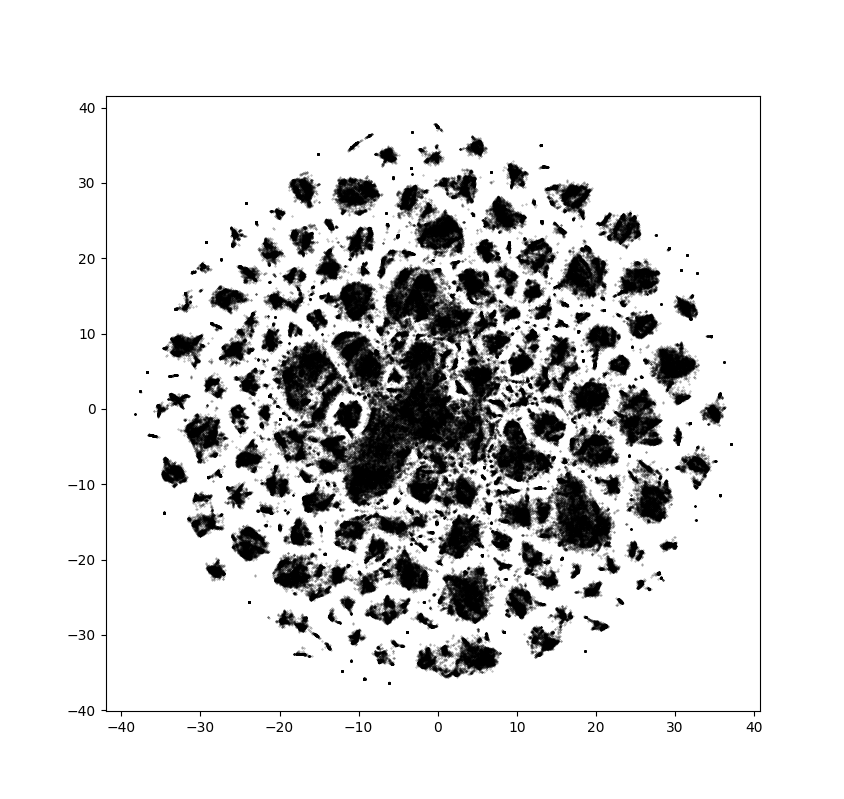
\includegraphics[width=1\textwidth]{images/tsne_clusters.png}
        \caption{tSNE plot from globo dataset}
        \label{fig:tsne_plot}
    \end{figure}

    \textbf{Affinity propagation.} The advantage of affinity propagation between other algorithms is that it does not need to specify an estimate of quantity of points found into the space, it naturally walks trough the points and finds the resulting clusters.

    On figure \ref{fig:affinity_twins} there is the visualization of the discovered clusters on the low dimensional embedding representation from tSNE result of globo dataset, the second image shows the center from each topic cluster, that later should be used to calculate the semantic difference from each topic based on the euclidean distance from the pair of topics being compared.
     
    \begin{figure}[H]
        \centering
        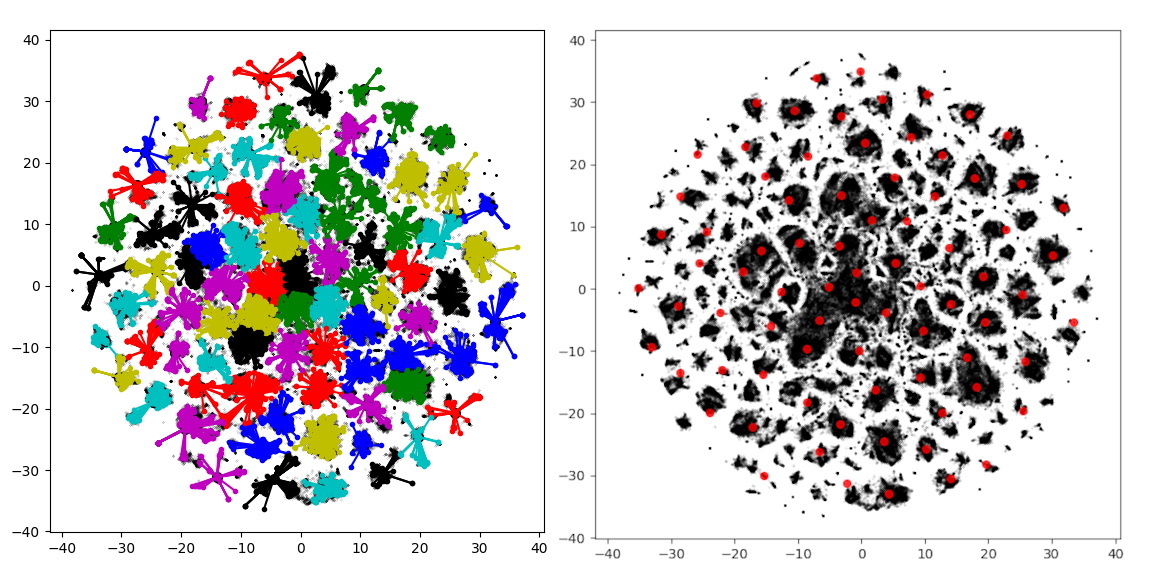
\includegraphics[width=1\textwidth]{images/affinity_twins.png}
        \caption{Affinity propagation clusters(left) and its centers(right)}
        \label{fig:affinity_twins}
    \end{figure}
    
    \textbf{Matrix Factorization.} Netflix is known for it's competitions for collaborative filters algorithms, in 2008 \textit{matrix factorization} \cite{srebro2004} was used and achieved a huge breakthrough in collaborative filtering algorithms, and it is like the prime factors for grown ups, using matrices as factors instead of just scalar numbers, it is a useful mechanism to separate the users-items matrix into a items' matrix and a users' matrix, that their multiplication result in the original users-items matrix, results into Item X User original association matrix that each item is the relation of one user to a single item.
    The usefulness of this factorization, is that since the original matrix is sparse, you can fill the missing values by making inferences on the factorized data, because not every user in its history has real relationship with every item.
    An optimal way of doing so is by using a modern version of \textit{Alternating Least Squares} algorithm \cite{takane1977} explained below that uses \textit{Gradient Descent} as convergence algorithm.
    
    
    \textbf{Alternating Least Squares.} It is a faster variant of the Matrix Factorization that allows it to be computational distributed, the as matrix factorization, it has SVD \cite{golub1971} as central role on the factorization between item and user matrices, but in this case, a cost function with an error function is alternated between each matrix, updating the elements of one matrix at a time, this computational behaviour reduces the complexity of the cost function and allows it to be computed in a distributed fashion.
    Today a common implementation of ALS is from Spark \(Hadoop\) in java, but also have facade libraries that allow calling ALS from spark \(Hadoop\) from other languages like Scala and Python (Pyspark).

    \section{Technology usage} \label{technology_usage}

    It was used \(Python3\) with \textit{pandas} \cite{reback2020pandas} and \textit{numpy} as main data manipulation, \(Pyspark\) was used for ALS method recommender system. 
    \(Pyspark\) is a python library that is a facade for a java spark hadoop spark application server that uses map/reduce in order to make distributed computations.

    For both tSNE and Affinity propagation \textit{sklearn} library was the choice and the source code from the proposed work is available at github \footnote{github.com/zatura/clickstream-content-sessionization}
        
        \subsection{Applying Dimensionality reduction}
        Because \textit{Globo.com} news text data is closed source, \cite{moreira2018chameleon} made available the trained article embeddings data \footnote{kaggle.com/gspmoreira/news-portal-user-interactions-by-globocom} generated from its unique \textit{CHAMALEON} RNN-based algorithm. The embedding file consists into a matrix of 250 dimensions of features and 364,047 news articles, those features are a representation of the content for each respective news article.
    
        On the proposed method only the following data and respective embedding were considered: \textit{click\_timestamp, article\_id} and \textit{{}user\_id}.
        
    
        Since on their work tSNE was mentioned as a good method for dimensionality reduction, tSNE was applied on the embedding, resulting into a pair of coordinates \(X, Y\) for each article id as the dataframe sample below:
        
        \begin{table}[H]
            \centering
            \begin{tabular}{ |c|c|c| } 
                \hline
                article\_id & x & y \\
                \hline 
                ... & ... & ... \\
                69 & 10.950659 & -26.211418 \\ 
                81 & 34.414822 & -0.690890 \\ 
                84 & 35.335995 & -1.578238 \\ 
                ... & ... & ... \\
                \hline
            \end{tabular}
            \caption{tSNE coordinate results}
            \label{tab:tsne_results}
        \end{table}
        
        \newpage
        
        \subsection{Applying Clustering}
        At this step, \textit{Affinity propagation} is applied on the tSNE result data plane, several damping parameters were tested and presented further at the error metrics section. 
        After the clustering, each cluster center point into the resulting plane receives a random generated human-readable label with the format \textit{<random\_color-random\_substantive>}, as shown on table \ref{tab:labeled_clusters} example, also, chart \ref{fig:benford} shows the distribution of consumed topics by a sampled user resembling a Benford's law distribution:
        
        
        \begin{table}[H]
            \centering
                \begin{tabular}{ |c|c|c| } 
                \hline
                x & y & topic \\
                \hline 
                ... & ...  & ... \\
                19.699291 & -28.117729 & tangerine-events \\ 
                -8.711248 & 21.906485 & purple-occurrences \\ 
                11.325381 & 3.893677 & yellow-episodes \\ 
                ... & ...  & ...  \\
                \hline
                \end{tabular}
            \caption{Labeled cluster centers}
            \label{tab:labeled_clusters}
        \end{table}
        
        \begin{figure}[H]
            \centering
            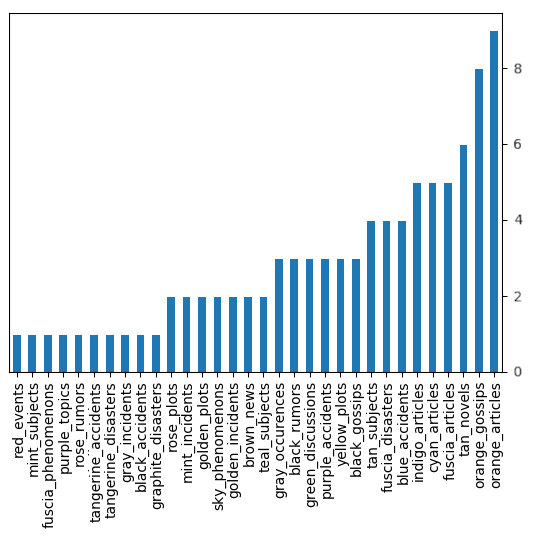
\includegraphics[width=0.8\textwidth]{images/benford.png}
            \caption{Topic frequencies from a sampled user}
            \label{fig:benford}
        \end{figure}

% =======================================================================

\chapter{Results} \label{results}

    Here there will be a comparison between \textit{euclidean distance} threshold against \textit{alternating least square} methods and its parameters variations, different combinations of items and sessions were performed like the impact of temporal ordering or shuffling items by timestamp, different affinity propagation damping factors and different sizes of sessions.
    
    On section \ref{globo_dot_com_dataset} Globo dataset properties are presented, on \ref{euclidean_distance_heuristic}, section \ref{session_simulation} the simulation of sessions as metric method is adressed with its results and on \ref{affinity_propagation_results} error heatmaps from iterations are shown.

    % TODO como foi separado test data vs non-test data, foi seguido o mesmo método do Zhang 1/4 vs 3/4??
    % TODO talvez seja interessante uma seção de performance(precision and recall) e limites do algoritmo (e do método de clusterização)
    % TODO seção pode ser chamada apenas de Datasets
    \section{Dataset} \label{globo_dot_com_dataset}
    %TODO contextualização disso nesse capítulo
    The dataset of choice was globo.com news dataset, it is a collection that consists on the following:
    \begin{itemize}
        \item approximately 2.8 millions news clicks
        \item more than 300 thousand users
        \item 45 thousand news articles
        \item 250 dimensional feature matrix
    \end{itemize}
    
    Since the availability of articles text data were not allowed by the company by commercial reasons, at \cite{moreira2018chameleon} presented CHAMELEON, a RNN algorithm for feature extraction, and together with the dataset, they made available a feature embeddings file extracted from its novel algorithm. Every news from the dataset have its own 250 feature dimensions on the embedding matrix
    
    The dataset consists on the following data for each click as the columns:
    
    \(user\_id, session\_id, session\_start, session\_size, click\_article\_id,\) 
    
    \(click\_timestamp, click\_environment, click\_deviceGroup, click\_os, \)
    
    \(click\_country, click\_region, click\_referrer\_type \)

    However session attributes such as \(session\_id, session\_start\) and \(session\_size\) are presented in the dataset, they were not considered on this session split method since they would conflict with the timeless nature approach, the only columns considered were \(click\_timestamp, user\_id\) and \(article\_id\) along with article embeddings; dataset sample is showed on the table below:
    
    \begin{table}[H]
        \centering
        \begin{tabular}{ |c|c|c|c|c|c|c|c|c|c| } 
            \hline
            click\_timestamp & user\_id & article\_id & click\_country & click\_region & ... \\
            \hline 
            ... & ...  & ...  & ...  & ... & \\
            1506826800026 & 59 & 234853 & 1 & 21 & \\ 
            1506826801702 & 79 & 159359 & 1 & 13 & ...\\ 
            1506826804207 & 154 & 96663 & 1 & 25 & \\ 
            ... & ...  & ...  & ...  & ... & \\
            \hline
        \end{tabular}
        \caption{Globo dataset sample as Dataframe}
        \label{tab:globo_dataset_sample}
    \end{table}


    \section{Evaluation metric} \label{euclidean_distance_heuristic}
    The chosen method for finding session boundaries was based on the will that users tend to encircle same or similar topics, similarly as shown on chart \ref{fig:benford}, on that sense, this hypothesis was used to create a model using euclidean distance from topics to measure how different they are.
    
    \begin{definition}
    In a session \(S\) with a set of items \(i_{1}, i_{2}, ...\) that each item has a \textit{topic} \(t\) associated, where each \textit{topic} \(t\) has a known coordinate \(x, y\) in a Cartesian plane.
    If the euclidean distance between the topic \(t_{p}\) of item \(i_{n}\) and the topic \(t_{q}\) of item \(i_{n+1}\) is higher than a chosen cutoff \(c\), than it is considered an end of a session and beginning of another.
    \label{euclidean_distance_threshold_definition}
    \end{definition}

    
    The error metrics from cutoff heuristic is defined as follow:
    
        
        \begin{itemize}
            \item The cutoff \(c\) is a row index that belongs to one of the sessions, this index is found by the cutoff trigger heuristic at definition \ref{euclidean_distance_threshold_definition}
            \item Because the two sessions doesn't have the same amount of items, thus asymmetric, a normalization mapping of the error metric is performed, the normalization effect is described on a gray color scale on table \ref{tab:cutoff_table}.
            \item It is calculated the difference between the number of items from the inferred index(found by heuristic) and the perfect index(the real cutoff) and divided by the total number of items at the artificial session (made by two real sessions), as represented above in the gray-colored table \ref{tab:cutoff_table} by the error column.
            
            So in this example, the index 3 is the perfect cutoff, representing the real threshold between the two sessions, the picked index by the cutoff heuristic will receive the respective error from its index row.
        \end{itemize} 
        
                    \begin{table}[H]
                \centering
                \begin{tabular}{c|c|c}
                    \hline
                    \rowcolor[RGB]{239,239,239}
                    index & user\_id & error \\
                    \hline 
                    \rowcolor[RGB]{140,140,140}
                    0 & 111 & 1 \\ 
                    \rowcolor[RGB]{197,197,197}
                    1 & 111 & 0.66 \\ 
                    \rowcolor[RGB]{226,226,226}
                    2 & 111 & 0.33 \\ 
                    \rowcolor[RGB]{255,255,255}
                    3 & 888 & 0 \\ 
                    \rowcolor[RGB]{239,239,239}
                    4 & 888 & 0.16 \\ 
                    \rowcolor[RGB]{222,222,222}
                    5 & 888 & 0.33 \\ 
                    \rowcolor[RGB]{206,206,206}
                    6 & 888 & 0.5 \\ 
                    \rowcolor[RGB]{189,189,189}
                    7 & 888 & 0.66 \\ 
                    \rowcolor[RGB]{173,173,173}
                    8 & 888 & 0.83 \\ 
                    \rowcolor[RGB]{140,140,140}
                    9 & 888 & 1 \\ 
                    \hline
                \end{tabular}
                \caption{Error normalization map from desired cutoff index}
                \label{tab:cutoff_table}
            \end{table}

        \section{Session simulation} \label{session_simulation}
        Because the dataset already have labeled the respective \textit{user id} in each row, it was considered that the most part of accounts were in fact from individual users, in that case, it is assumed that even if some users really share the same account, this would be statistically irrelevant when analyzing the whole dataset.
        Considering this scenario true, the simulated sessions is constructed as a concatenation of two streams of two separated user ids 
        as addressed on table \ref{session_simulation} a sample from a simulated session.
        
        Notice that the column \textit{distance} stands for euclidean distance from current centroid of row index \(n\) and centroid from row index \(n - 1\) in a simulated session table.
        
        \begin{table}[H]
            \centering
            \begin{tabular}{ |c|c|c|c|c|c| } 
                \hline
                \  & click\_timestamp & user\_id & x\_centroid & y\_centroid & distance \\
                \hline 
                 ... & ... & ... & ... & ... & ... \\
                 11 & 1507987156229 & 6207 & -8.487595 & 3.206146 & 43.517998 \\
                 12 & 1507988999717 & 6207 & 3.864952 & -3.751176 & 27.925744 \\
                 13 & 1507989029717 & 6207 & 5.004131 & 3.442250 & 7.283071 \\
                 \rowcolor[RGB]{220,220,220}
                 14 & 1507061447189 & 143259 & 25.503668 & -1.358489 & 21.054171 \\
                 15 & 1507061615464 & 143259 & 18.530073 & -15.994876 & 16.212799 \\
                 16 & 1507061615464 & 143259 & 18.530073 & -15.994876 & 0.000000 \\
                 ... & ... & ... & ... & ... & ... \\
                \hline
            \end{tabular}
            \caption{Simulated session sample with desired cut in gray}
            \label{tab:session_simulation}
        \end{table}
        
        \section{Temporal desambiguation} \label{temporal_ordering_factor}
        
        Since time ordering can be sensitive for news articles a method to disambiguate the influence of temporal order was introduced because the objective of this work is to segregate sessions exclusively on its content excluding time factor for example.
        
        There were two different types of measurements, one of them had time ordering were each user session had its items ordered by its timestamp, on the second one, the items were completely shuffled, removing time influence.
        
        A floor cutoff euclidean distance was pick as 1, and the ceiling as 60, the origin of those numbers is related to the scale of de tSNE plot addressed on figure \ref{fig:tsne_plot}. With this limits defined, 15 linearly spaced cutoff distances were generated as input as shown by columns \textit{cutoff dist} on table \ref{tab:cutoff_timestamp_ordered_shuffled}, for each session cut attempt, an error were calculated and attributed as section \ref{euclidean_distance_heuristic} describes, an array of error metrics was created and an \textit{error mean} and also an \textit{error standard deviation}, described on second and third column of table \ref{tab:cutoff_timestamp_ordered_shuffled}.
        
        Looking on both mean and std metrics result, it has a neat meaning that time order does not affect the euclidean threshold heuristic, however, it is important to notice the high error mean (more than 0.5), furthermore, the results shows that the lower the error mean, the error standard deviation rises considerably, thus making it less reliable. For example, on table \ref{tab:cutoff_timestamp_ordered_shuffled}, notice that on the table with time ordering, the lowest error mean is 0.611 and its standard deviation mean is 0.3 or in other words, a deviation of 30 \%, making this cutoff parameter unreliable for the session cutting purpose.
        
        \begin{table}[H]
        \centering
        \subfloat[\label{ordered}]{
            \begin{tabular}{ |c|c|c| } 
                \hline
                cutoff dist. & error mean & error std \\
                \hline 
                1.00 & 0.933 & 0.053 \\
                5.21 & 0.932 & 0.054 \\
                9.42 & 0.922 & 0.071 \\
                13.64 & 0.917 & 0.078 \\
                17.85 & 0.901 & 0.098 \\
                22.07 & 0.877 & 0.126 \\
                26.28 & 0.857 & 0.151 \\
                30.5 & 0.812 & 0.191 \\
                34.71 & 0.765 & 0.230 \\
                38.92 & 0.681 & 0.266 \\
                43.14 & 0.629 & 0.286 \\
                43.35 & 0.611 & 0.301 \\
                51.57 & 0.630 & 0.311 \\
                55.78 & 0.707 & 0.320 \\
                60.00 & 0.814 & 0.287 \\
                \hline
            \end{tabular}
        }
        \rule{1cm}{0cm}
        \subfloat[\label{shuffled}]{
            \begin{tabular}{ |c|c|c| } 
                \hline
                cutoff dist. & error mean & error std \\
                \hline 
                1.00 & 0.939 & 0.045 \\
                5.21 & 0.938 & 0.048 \\
                9.42 & 0.933 & 0.057 \\
                13.64 & 0.927 & 0.663 \\
                17.85 & 0.912 & 0.088 \\
                22.07 & 0.893 & 0.114 \\
                26.28 & 0.867 & 0.144 \\
                30.5 & 0.827 & 0.184 \\
                34.71 & 0.778 & 0.223 \\
                38.92 & 0.710 & 0.264 \\
                43.14 & 0.646 & 0.289 \\
                43.35 & 0.615 & 0.310 \\
                51.57 & 0.631 & 0.322 \\
                55.78 & 0.721 & 0.325 \\
                60.00 & 0.813 & 0.298 \\
                \hline
            \end{tabular}
        }
        \caption{Error metrics, session ordered by timestamp \ref{ordered} vs shuffled \ref{shuffled} }
        \label{tab:cutoff_timestamp_ordered_shuffled}
        \end{table}
    
    \section{Affinity propagation damping factor} \label{affinity_propagation_results}
        Another possibility for interference on session cuts performance can be the granularity of clustering, or in other words, how specific or generic that a topic classification should be so that it is enough to recognize the difference between users sharing an account? 
        
        In a single topic like Math, many areas can be classified like algebra, calculus, statistic and so on, at the same time, you can be more generic, and simply address that all those areas are simply Math, and then you segregate other topics as Portuguese, Biology, Math and so on without opening into details.
        
        Since the \textit{damping factor} from the Affinity Propagation Algorithm described on section \ref{algorithms} changes the amount of classified clusters, another parameter was introduced on the error metrics calculations and that being the \textit{damping factor}. For different damping factors, the amount of topics is addressed on table \ref{tab:damping_factor}.

        \begin{table}[H]
            \centering
            \begin{small}
                \begin{tabular}{ |c|c| } 
                    \hline
                    damping & nº of clusters \\
                    \hline 
                    0.5 & 4771 \\ 
                    0.553 & 4716 \\ 
                    0.606 & 2984 \\
                    0.66 & 1146 \\
                    0.766 & 91 \\
                    0.82 & 152 \\
                    \hline
                \end{tabular}
                \end{small}
            \caption{damping factor effect on nº of clusters}
            \label{tab:damping_factor}
        \end{table}
        
        Similarly as section \ref{temporal_ordering_factor} a number of 15 cutoff values were tested between values 1 and 60, linearly spaced for each iteration with a different cutoff . The output was a vector of error values of the same size of the simulated sessions (one for each session, about 32 thousand sessions).
        Then, from this error vector, it was calculated its mean and standard deviation for each iteration (15 iterations), so that we could measure its reliability and precision.
        
        The error heatmaps results are interpreted as the following:
        \begin{itemize}
            \item The Vertical axis of the represents the affinity propagation damping factor
            \item The Horizontal axis corresponds to the chosen cutoff distance threshold
            \item the value of each item on the heatmap corresponds to one of two metric errors: Mean error, Standard deviation error.
        \end{itemize}
    
        The objective of this metric is finding a lower than 50\% mean error and the lowest \(standard\ deviation\).
        
        % TODO explicar resultados, foram bons? foram ruins?
        \begin{figure}[htp]
            \centering
            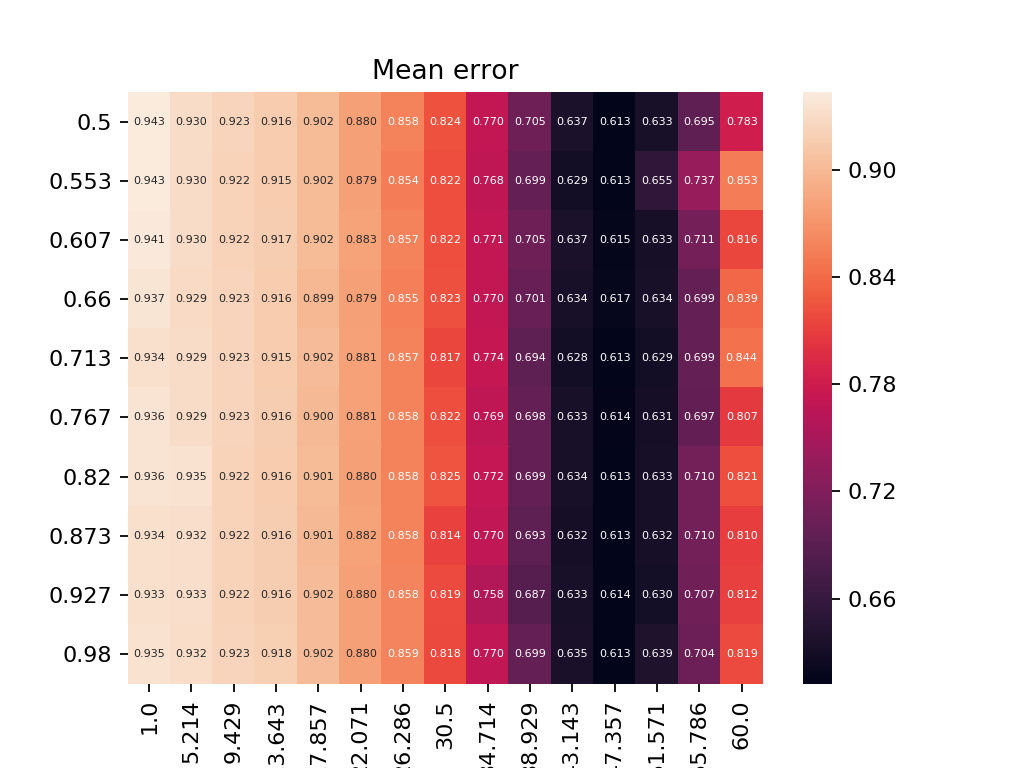
\includegraphics[width=0.95\textwidth]{images/error_mean.png}
            \caption{Error mean heatmap}
            \label{fig:error_mean_heatmap}
        \end{figure}
        
        \begin{figure}[htp]
            \centering
            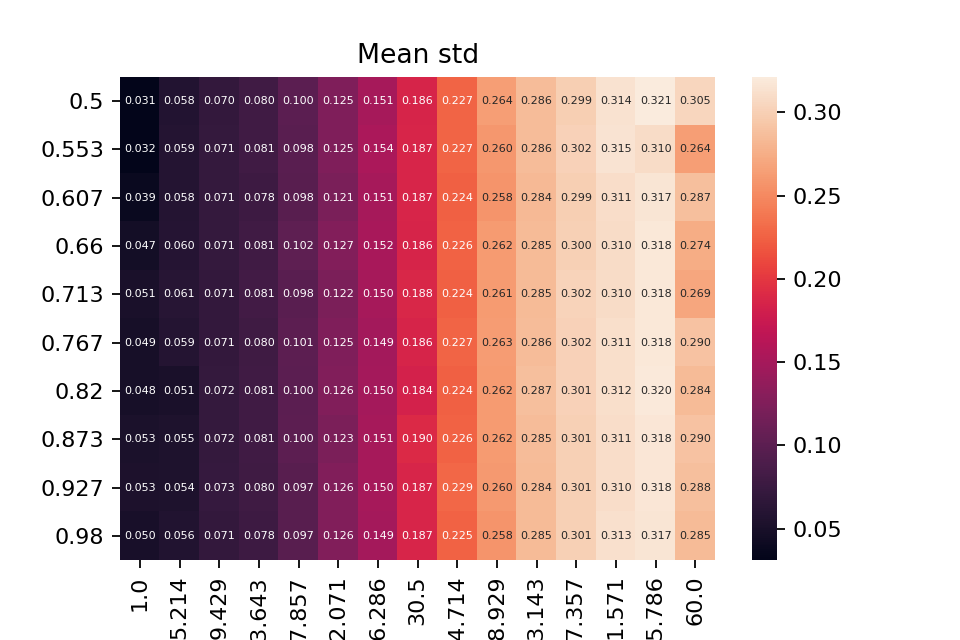
\includegraphics[width=0.98\textwidth]{images/error_std.png}
            \caption{Error standard deviation heatmap}
            \label{fig:error_std_heatmap}
        \end{figure}
    
    \newpage     
    \section{Alternating least squares comparison}
        
        The last attempt to verify the reliability of the session cutoff method was using topic read frequency per user and feeding into an ALS implicit recommender system using \textit{pyspark}, mentioned on section \ref{technology_usage}, creating a list of sets \((user\_id, topic\_alias, read\_frequency)\) as shown on table \ref{tab:als_read_frequency}. Later, data was split into 25\% / 75\% train vs test data and the ALS model was trained.
        
        \begin{table}[H]
            \centering
            \begin{tabular}{ |c|c|c| } 
                \hline
                user\_id & topic\_alias & read\_frequency \\
                \hline 
                ... & ... & ... \\
                26340 & purple-articles & 7 \\ 
                26340 & rose-stories & 5 \\ 
                58277 & cyan-contents & 1 \\ 
                ... & ... & ... \\
                \hline
            \end{tabular}
            \caption{ALS: Read frequency per topic}
            \label{tab:als_read_frequency}
        \end{table}
        
        In order to avoid cold start, only users with more than 200 items in total were chosen.
        Same as Euclidean Distance experiment on \ref{euclidean_distance_heuristic}, fictitious sessions were created, but instead of a distance column as error metric, a new column 'prediction' were added that corresponds to the predicted probability that the probe \(user\_id\) is likely to read that article.

        The next step relies on making a cross probing between a pair of user sessions each time, so in a session from \(user\_id = 413\), the predicted probability for each item is calculated for \(user\_id = 45502\), than it is calculated the \textit{mean} of all predictions as well as its \textit{standard deviation} as shown on second line of table \ref{tab:alternate_least_squares_metrics}, lastly, the process is repeated with the \(user\_id = 413\) against itself. The expectation of this experiment is that the prediction\_mean of an user session comparing against itself should be high at majority of times with low \textit{standard deviation} and for the second user session against the first one, the prediction\_mean for the second user against the first should be at some median value with high \textit{standard deviation}, meaning less correlation.
        
        However, looking at table \ref{tab:alternate_least_squares_metrics} there seems to be no relevant difference between the \textit{prediction means} and \textit{prediction standard deviations}, meaning that results from previous steps or even the embeddings could be faulty at some point.

        
        \newpage 

        The following table was created as result, it was extracted metrics from 413 users.
        \begin{table}[H]
            \centering
            \begin{tabular}{ |c|c|c|c| } 
                \hline
                user\_id & user\_id\_to\_predict & prediction\_mean & prediction\_std \\
                \hline 
                413 & 413 & 0.83287 & 0.2799 \\
                45502 & 413 & 0.86549 & 0.25900 \\
                \rowcolor[RGB]{220,220,220}
                12897 & 12897 & 0.84201 & 0.3291 \\
                \rowcolor[RGB]{220,220,220}        
                16695 & 12897 & 0.91515 & 0.27717 \\
                2930 & 2930 & 0.79370 & 0.34552 \\
                9261 & 2930 & 0.87126 & 0.2551 \\
                \rowcolor[RGB]{220,220,220}        
                20001 & 20001 & 0.8777 & 0.24580 \\
                \rowcolor[RGB]{220,220,220}        
                6344 & 20001 & 0.91090 & 0.2383 \\
                62025 & 62025 & 0.75506 & 0.35445 \\
                19864 & 62025 & 0.47764 & 0.27196 \\
                \rowcolor[RGB]{220,220,220}        
                43017 & 43017 & 0.83342 & 0.27467 \\
                \rowcolor[RGB]{220,220,220}        
                21356 & 43017 & 0.81031 & 0.28030 \\
                3391 & 3391 & 0.85998 & 0.2949 \\
                681 & 3391 & 0.87366 & 0.30739 \\
                \rowcolor[RGB]{220,220,220}        
                11521 & 11521 & 0.61621 & 0.3742 \\
                \rowcolor[RGB]{220,220,220}                
                59193 & 11521 & 1.01384 & 0.5024 \\
                11359 & 11359 & 0.88445 & 0.2596 \\
                23036 & 11359 & 0.91379 & 0.24409 \\
                \rowcolor[RGB]{220,220,220}                
                22301 & 22301 & 0.81135 & 0.30362 \\
                \rowcolor[RGB]{220,220,220}                
                77985 & 22301 & 0.78393 & 0.32523 \\
                13885 & 13885 & 0.85638 & 0.264 \\
                9193 & 13885 & 0.80591 & 0.2890 \\
                \hline
            \end{tabular}
            \caption{Alternating Least Squares measurements}
            \label{tab:alternate_least_squares_metrics}
        \end{table}

% =======================================================================

\chapter{Conclusion}
% Given the event-driven nature of news
The error standard deviation presented on the heatmaps with different input parameters reveals that the euclidean distance as threshold method does not have enough precision, but these results could have many explanations not only from the method itself. Since globo dataset is closed source and the embedding features available from \cite{moreira2018chameleon} were created from his own algorithm, a certain level of belief was implied that the embeddings really reflected its content and his algorithm worked well on quantitatively describing them.

The ALS algorithm method evaluation showed that there were no relevant item similarity between users itself against other users, meaning that rather this is a cause of the chaotic nature of news or tSNE as dimensionality reduction wasn't precise enough to classify the different news topics.

%TODO talk about the flaw of this method, like users with same interest sharing account 
Finally, news as a type of media have event-driven and chaotic nature, even when readers have his preference for certain topics, unexpected and relevant news from other topics may arrive and catch the readers eyes, those phenomena are maybe common, thus, the proposed method of sessionization by euclidean distance is not a good candidate to split sessions based on its content.


\bibliographystyle{packages/abntex2-alf}
\bibliography{biblio}

\end{document}
